\documentclass[a4paper,10pt]{article}
\usepackage[left=1in, right=.8in,top=1in, bottom=.8in]{geometry}



%A Few Useful Packages
\usepackage{marvosym}
\usepackage{fontspec} 					%for loading fonts
\usepackage{xunicode,xltxtra,url,parskip} 	%other packages for formatting
\RequirePackage{color,graphicx}
\usepackage[usenames,dvipsnames]{xcolor}
%\usepackage[big,binding=-.5cm]{layaureo} 				%better formatting of the A4 page
% an alternative to Layaureo can be ** \usepackage{fullpage} **
\usepackage{titlesec}					%custom \section

\usepackage{tabularx} 
\usepackage{tabu}
\usepackage{ltablex}

\usepackage[none]{hyphenat}

\usepackage{booktabs}% http://ctan.org/pkg/booktabs
\newcommand{\tabitem}{~~\llap{\textbullet}~~}

\usepackage{multirow}

%Setup hyperref package, and colours for links
\usepackage{hyperref}
%\definecolor{linkcolour}{rgb}{0,0.2,0.6}
\definecolor{linkcolour}{rgb}{0,0,0}
\hypersetup{colorlinks,breaklinks,urlcolor=linkcolour, linkcolor=linkcolour}

%FONTS
\defaultfontfeatures{Mapping=tex-text}
%\setmainfont[SmallCapsFont = Fontin SmallCaps]{Fontin}
%%% modified for Karol Kozioł for ShareLaTeX use
\setmainfont[
SmallCapsFont = Fontin-SmallCaps.otf,
BoldFont = Fontin-Bold.otf,
ItalicFont = Fontin-Italic.otf
]
{Fontin.otf}
%%%

%CV Sections inspired by: 
%http://stefano.italians.nl/archives/26
\titleformat{\section}{\Large\scshape\raggedright}{}{0em}{}[\titlerule]
\titlespacing{\section}{0pt}{3pt}{3pt}
%\titleformat{\section}[display]
%{\Large\scshape\raggedright}{}{0pt}{}[\titlerule] 
%Tweak a bit the top margin
%\addtolength{\voffset}{-1.3cm}

%Italian hyphenation for the word: ''corporations''
\hyphenation{im-pre-se}

%-------------WATERMARK TEST [**not part of a CV**]---------------
\usepackage[absolute]{textpos}

\setlength{\TPHorizModule}{30mm}
\setlength{\TPVertModule}{\TPHorizModule}
\textblockorigin{2mm}{0.65\paperheight}
\setlength{\parindent}{0pt}

%--------------------BEGIN DOCUMENT----------------------
\begin{document}

\pagestyle{empty} % non-numbered pages

\font\fb=''[cmr10]'' %for use with \LaTeX command

%--------------------TITLE-------------
%\par{\centering
		%{\Huge Seyed Jalal \textsc{Hosseini}
	%}\bigskip\par}

%--------------------SECTIONS-----------------------------------
%Section: Personal Data
%\section{Personal Data}

\begin{tabular}{rll}
    \multicolumn{2}{l}{\LARGE Seyed Jalal Hosseini} &
    \multirow{5}{*}{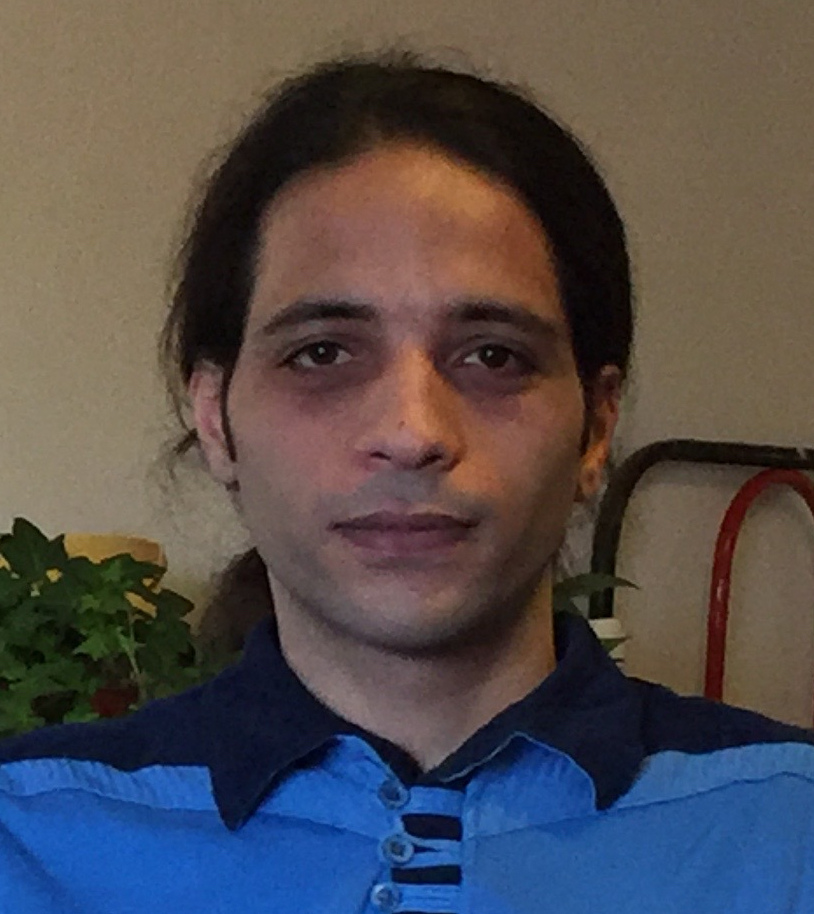
\includegraphics[width=30mm]{img/img02.jpg}}\\[1.3ex]
    \textsc{Place and Date of Birth:} & Tehran, Iran  | 1st March 1987 &\\
    \textsc{Address:}   & Via D'Azeglio 23, 40123, Bologna, Italy &\\
    \textsc{Phone:}     & +39 392 5036611&\\
    \textsc{email:}     & \href{mailto:jalalhosseiny@gmail.com}{jalalhosseiny@gmail.com}&\\
    \textsc{github:}     & \href{https://github.com/artronics}{artronics}&
\end{tabular}

%Summary section. Look for summary dir to import one
\section{Summary}
\nohyphens{\justify
An \textbf{Embedded System Engineer} with expertize in \textbf{Hardware Design} and \textbf{Software Development}. Experienced in \textbf{Linux},
and low-level programming in \textbf{C} and \textbf{Assembly}, with comprehensive knowlodge in high-level
enterprise software development, \textbf{OOP}, \textbf{TDD} and Open Source solutions and hands on experience in front end development,
familiar with \textbf{Javascript, HTML} and \textbf{CSS}. Provides end-to-end solutions from HW prototyping to SW implementation.
}


%Section: Education
\section{Education}
    \begin{tabu}{X | X[7]}    
	\textsc{March} 2016 & \textbf{M.Sc} in \textbf{Telecommunication Engineering}, \textbf{Universiy of Bologna}, Bologna\\
    & Thesis: ``\textbf{Software-Defined Wireless Sensor Networks}'' \\& \small Advisor: Prof. Roberto \textsc{Verdone} | \normalsize \textsc{Gpa}: 100/110\\\multicolumn{2}{c}{} \\
	\textsc{Fall} 2010& \textbf{B.Sc} in \textbf{Telecommunication and Electronics Engineering}, \normalsize\textbf{University of Zanjan}, Zanjan\\
    & Thesis: ``\textbf{Motion Controlled Robotic Arm}''
\end{tabu}

%Section: Work Experience at the top
\section{Work Experience}

    \begin{tabu}{X | X[7]}    
    \emph{2012} & \textbf{Technical Telecommunication Consultant} at \textbf{IGS}, \textsc{Shahid Rajaee Port Complex} \\
    \textsc{2011}& 
  \small \textbullet~Consulting on supplying equipment and spare parts\normalsize \\&
  \small \textbullet~Equipment maintenance, consultant and inspector\normalsize\\
 \multicolumn{2}{c}{} \\
 
    \emph{2011} & \textbf{Embedded System Engineer} at \textbf{Mobtakeran Fan Nab Co}, \textsc{Tehran, } \\\textsc{2010}&
  \small\textbullet~Consulting on Industrial Projects\normalsize\\&
  \small\textbullet~Design, Simulation and Verification of projects\normalsize\\
  \multicolumn{2}{c}{} \\
    
\end{tabu}

\section{Technical Skills}
\begin{tabularx}{\textwidth}{p{\textwidth/7} p{\textwidth*6/7}}
 Programming Languages:& \textsc{Java}, \textsc{c++}, \textsc{c}, \textsc{c\#}, Assembly, \textsc{php}, Javascript\\&
 \footnotesize{\textbullet~\textbf{Full-Stack Developer} with high expertise in backend technologies}\\&
 \footnotesize{\textbullet~Complete knowledge of \textbf{Object Oriented Programming} and \textbf{Design Patterns}}\\&
 \footnotesize{\textbullet~Understanding of \textbf{Unit Testing,} \textbf{Source Control} and \textbf{Documentation}}\\&
 \footnotesize{\textbullet~Familiar with \textbf{Relational Database,} \textbf{MySQL, SQL Server} and \textbf{ORM} frameworks}
 \\\multicolumn{2}{c}{} \\
 
Operating Systems:& Windows,OS X, Unix/Linux\\&
 \footnotesize{\textbullet~Skilled in Linux Command Line and Bash scripting}\\&
 \footnotesize{\textbullet~Virtualization: \textbf{Vagrant, VMWare, qemu}}\\&
 \footnotesize{\textbullet~Source Control Management: \textbf{git}}\\&
 \footnotesize{\textbullet~Server Administration: \textbf{apache, nginx, mysql}}\\&
 \footnotesize{\textbullet~Understanding of \textbf{signals, filesystems,} and \textbf{system calls}}
 \\\multicolumn{2}{c}{} \\

Embedded Systems:& ARM, AVR, PIC, Single Board Computers\\&
 \footnotesize{\textbullet~8-bit Microcontroller \textbf{AVR} megaAVR and XMEGA, \textbf{PIC} PIC12 and PIC16}\\&
 \footnotesize{\textbullet~32-bit Microcontroller \textbf{ARM} ARMv6-M, ARMv7-M, skilled in \textbf{Assembly} language}\\&
 \footnotesize{\textbullet~Software solution based on Linux Distribution on SBCs, hands on experience in \textbf{raspberry pi, Beagle Bone, mini2440}}
  \\\multicolumn{2}{c}{} \\
 
Simulation and CAD:& Altium Designer, Proteus, Vivado, OrCAD, Modelsim, VHDL\\&
 \footnotesize{\textbullet~End-to-end Embedded Systems design from \textbf{PCB} to \textbf{Test} and \textbf{Verification}}\\&
 \footnotesize{\textbullet~Skilled in Multilayer \textbf{PCB} design using \textbf{Altium Designer}}\\&
 \footnotesize{\textbullet~Advance \textbf{Microcontroller} simulation with \textbf{Proteus}}\\&
 \footnotesize{\textbullet~Familiar with \textbf{FPGA} design process: \textbf{VHDL},\textbf{Vivado}, \textbf{Xilinx} Spartan-6}
 \\\multicolumn{2}{c}{} \\
\end{tabularx}



\section{Projects}
\begin{tabu}{X X[7]}    
    Title & \large Software-Defined Wireless Sensor Networks (SDWSN) \\[.3ex]

    Description& \small This project brings \textbf{Software-Defined Networking (SDN)} concepts in to \textbf{Wireless Sensor Networks (WSNs)}. A \textbf{Client-Server} model connects each separated WSN to a \textbf{Centralized Controller} located in the Server. Client program exposes \textbf{REST} APIs to access Controller's resources. A \textbf{Single Page Application (SPA)} written in javascript \textbf{(Angularjs)} is in charge of monitoring the whole network.\normalsize\\&\\
    Significance & 
    \small\textbullet~Highly modular and loosely coupled design, written in Java.\normalsize\\&
    \small\textbullet~Cetralized Controller and Database.\normalsize\\&
    \small\textbullet~Clean and robust code; more than 200 unit tests with code coverage up to 80 percent\normalsize
\end{tabu}

\begin{tabu}{X X[7]}    
    Title & \large Motion Controlled Robotic Arm\\[.3ex]
    Description & \small A \textbf{servo robotic arm} which is controlled by analyzing potentiometer sensors signals attached to human arm. The system utilizes an \textbf{ARM Cortex-M3} board running \textbf{uC/OS-II}. Fixed number of real-time processes are executing controll algorithms.\normalsize\\&\\
    Significance &
    \small\textbullet~Enhance existing MATLAB controll procedures and algorithms to C code\normalsize\\&
    \small\textbullet~Design and create a prototype of the system\normalsize\\&
    \small\textbullet~Real-Time task scheduler with uC/OS-II\normalsize
\end{tabu}

\begin{tabu}{X X[7]}    
    Title & \large CAN Controller Module\\[.3ex]
    Description & \small This project provides an expandable communication interface in order to add/remove floors to an existing elevator controll board. The main bord communicates with different modules via CAN protocol.\normalsize\\&\\
    Significance &
    \small\textbullet~Cost-effective and maintainable solution for expandign current elevator infrastructure\normalsize\\&
    \small\textbullet~Using \textbf{MCP2515} CAN Controller with \textbf{MCP2552} CAN Tranceiver\normalsize\\&
    \small\textbullet~Using \textbf{PIC18F} microcontroller to drive CAN protocol and communicate with controller board\normalsize
\end{tabu}


%Section: Languages
\section{Languages}
\begin{tabular}{rl}
	\textsc{Farsi (Persian):}&Native\\
    \textsc{English:}&Fluent\\
    \textsc{Italian}& Elementary\\
    \textsc{Arabic}& Intermediate
\end{tabular}

\section{Interests and Activities}
Programming, Open Source enthusiast\\
Music, Travelling

\end{document}
